\documentclass[12pt]{amsart}
%%
\usepackage{microtype}
\usepackage{amsmath,amssymb}
\usepackage{array,delarray}
\usepackage[dvips]{graphicx} \usepackage{xspace}
\usepackage{wrapfig}
\usepackage{color}
\usepackage[square,sort&compress,numbers]{natbib}
\usepackage{times}
%\usepackage{caption}
\usepackage{subfig}
%\usepackage{subcaption}
\usepackage{colortbl}
\usepackage[table]{xcolor}
\usepackage{url}
\usepackage{microtype}

\usepackage{hyperref}
\hypersetup{colorlinks=true,linkcolor=blue,linkcolor=blue,citecolor=blue,urlcolor=blue}

%%
\graphicspath{{./}{./figs/}}

%%\usepackage{citesort}
%\usepackage{sidecap}
%\usepackage{times} % assumes new font selection scheme installed
%\usepackage[small]{caption}


\usepackage[colorinlistoftodos]{todonotes}
\newcommand{\TODO}[1]{\todo[inline,color=red!20,size=\small]{#1}}
\newcommand{\aacomment}[1]{({\color{magenta}AA: #1})}



\renewcommand{\thesection}{\Roman{section}}
%%\renewcommand{\thesubsection}{\thesection.\Alph{subsection}}
\renewcommand{\thesubsection}{{\bfseries\Alph{subsection}}}

%%
%%
\renewcommand\labelitemi{\rule[0.12em]{0.4em}{0.4em}}
\renewcommand\labelitemii{\normalfont\bfseries
  \rule[0.15em]{0.3em}{0.3em}}
\renewcommand\labelitemiii{\textasteriskcentered}
\renewcommand\labelitemiv{\textperiodcentered}
%%
%%
\newtheorem{theorem}{Theorem}[section] % Numbered within each section
\newtheorem{corollary}[theorem]{Corollary} % Numbered along with thm
\newtheorem{lemma}[theorem]{Lemma} % Numbered along with thm
\newtheorem{proposition}[theorem]{Proposition} % Numbered along with  thm
\theoremstyle{definition}
\newtheorem{definition}[theorem]{Definition} % Numbered along with thm
\theoremstyle{remark} \newtheorem{remark}[theorem]{Remark} % Numbered along with thm
\newtheorem{example}[theorem]{Example} % Numbered along with thm
\numberwithin{equation}{section} % Number equations within sections
%%
%% 8.5 x 11 with 1 inch margins all over.
\setlength{\captionindent}{1.0pc}
\usepackage[left=1.00in,top=1.00in,right=1.00in,bottom=1.00in,headheight=39pt,headsep=2pt]{geometry}
\usepackage{fancyhdr}


\parskip6pt
\parindent0pt

%% ----------------------------------------------------------------------

\def\twitter{Twitter\xspace}
\def\prob{\mathrm{Pr}}
\def\npsonesystem{NPS-1\xspace}
\def\taskname#1{\textbf{#1}}
%% ----------------------------------------------------------------------

\def\title{Creating synthetic distribution networks}

\pagestyle{fancy}
\fancyhead{}
\fancyfoot{}
%%\renewcommand{\headrulewidth}{0.4pt}
\fancyfoot[C]{\rlap{\phantom{$\int$}}\thepage}
\fancyhead[L]{{\small\hbox{\title}}}

%% ----------------------------------------------------------------------

\def\itemsym{\par\rule[0.5mm]{2mm}{2mm}\xspace\hangindent=12pt}
\def\itemnum#1{\par#1\xspace\hangindent=12pt}
%%
\begin{document}
	\thispagestyle{fancy} \phantom{}
	The previously proposed algorithm evaluated the mapping between road network nodes and house/activity locations based on the Voronoi regions generated by the road nodes. Then, it considered preordered traversals through the road network nodes which are mapped to at least one house/activity location. Thereafter, the substations were mapped to the preordered list of road nodes which belong to their Voronoi region.
	
	The algorithm generated a radial distribution network which is similar to a realistic representation of the distribution system. However, only the road nodes which are mapped to at least one house/activity location is included in the distribution network. For example, Fig.\ref{fig:1} shows the resulting synthetic distribution network generated using the previous algorithm for the substation with ID $34816$. The red lines indicate the distribution network while the blue dotted lines represent the road network.
	\begin{figure}
		\centering
		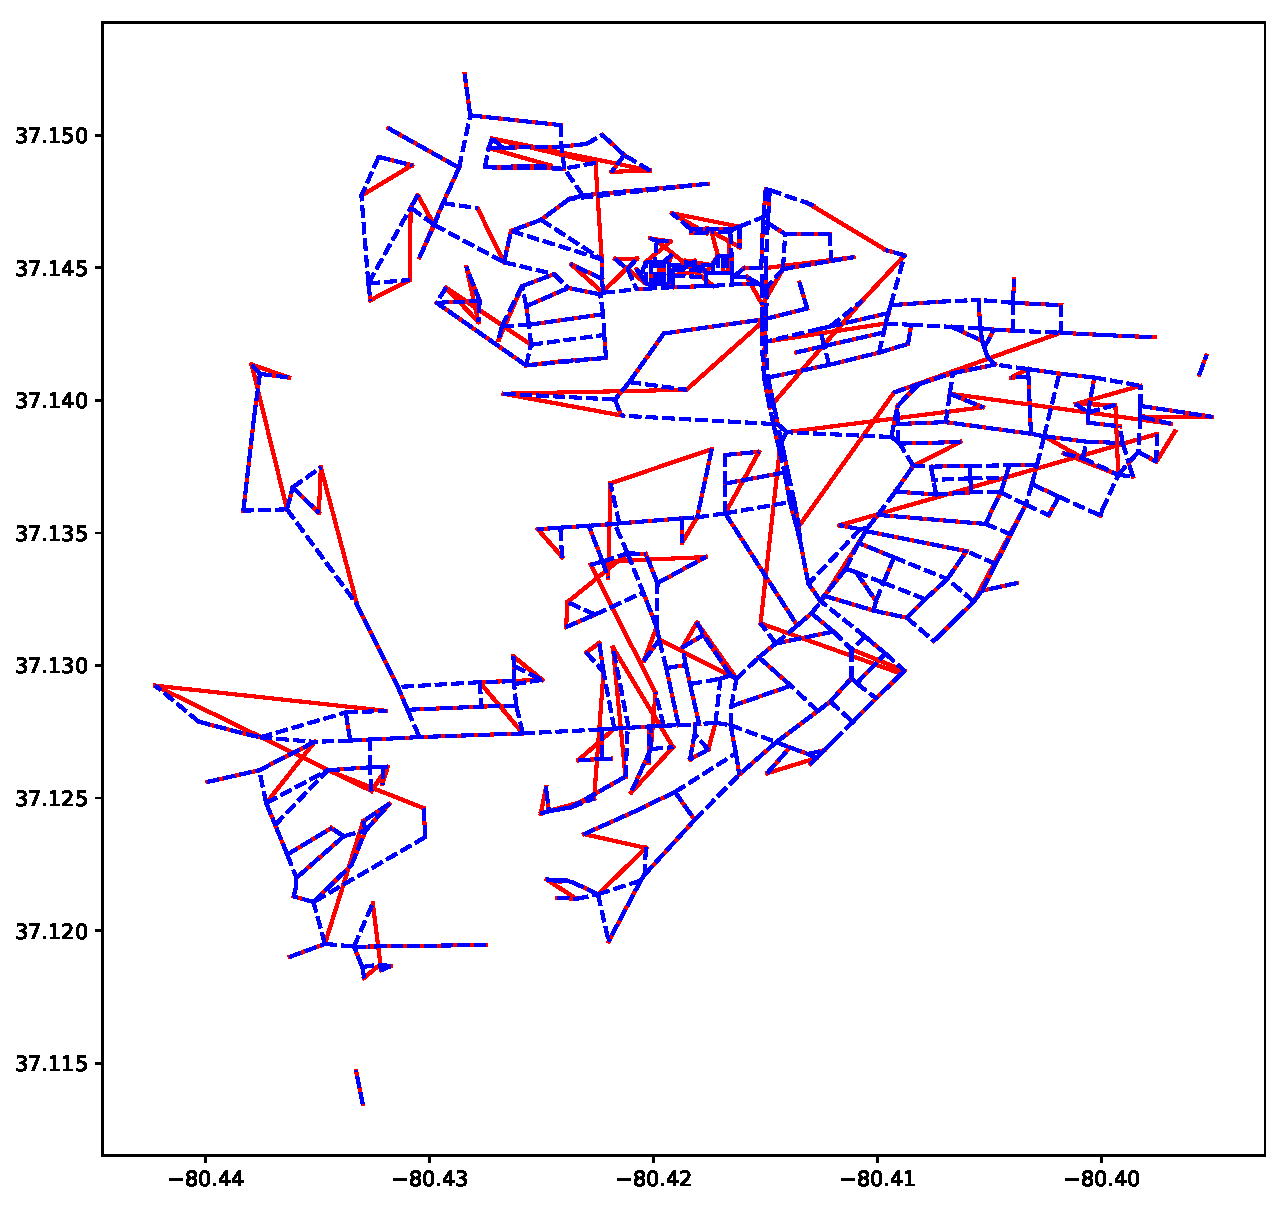
\includegraphics[scale=0.4]{figs/fig1.pdf}
		\caption{Synthetic distribution network created using previous algorithm}
		\label{fig:1}
	\end{figure}
	
	It is observed from Fig.\ref{fig:1} that the distribution network has deviated from the road network to a great extent. In practice, the distribution lines are either overhead with electric poles placed along the roadways or underground and installed in trenches alongside roads. Therefore, the synthetic network generated does not produce a realistic representation of the distribution system. 
	
	In order to make the distribution network follow the roadways to the maximum extent possible, the road network can itself be used to generate the synthetic distribution system. First, the road nodes and home/activity locations can be mapped to the Voronoi region of each substation. Then the road network can be converted to a tree structure (using depth-first search algorithm) to represent the distribution network. Fig.\ref{fig:2} shows the distribution system generated using this approach for the substation with ID $34816$. In the left figure, the red lines indicate the road network formed with all the road nodes in the Voronoi region of the substation and the blue circles represent the home/activity locations in it. The green circle represents the substation. In the right figure, the road network has been converted to a radial (tree structure) distribution system.
	\begin{figure}
		\centering
		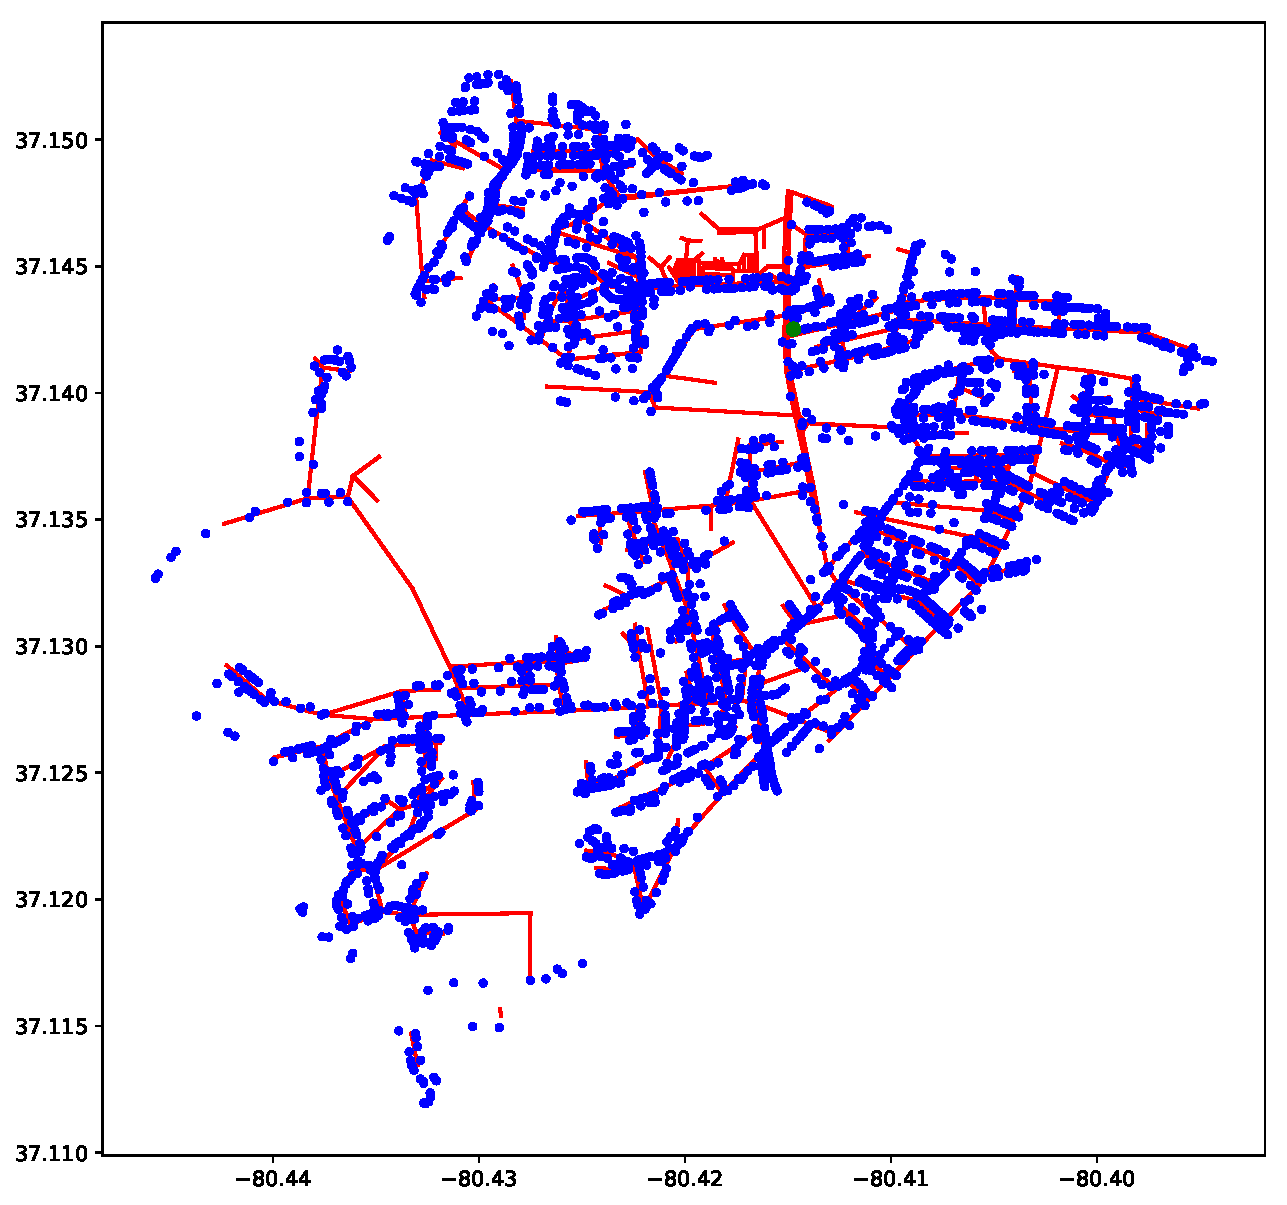
\includegraphics[scale=0.35]{figs/fig2a.pdf}
		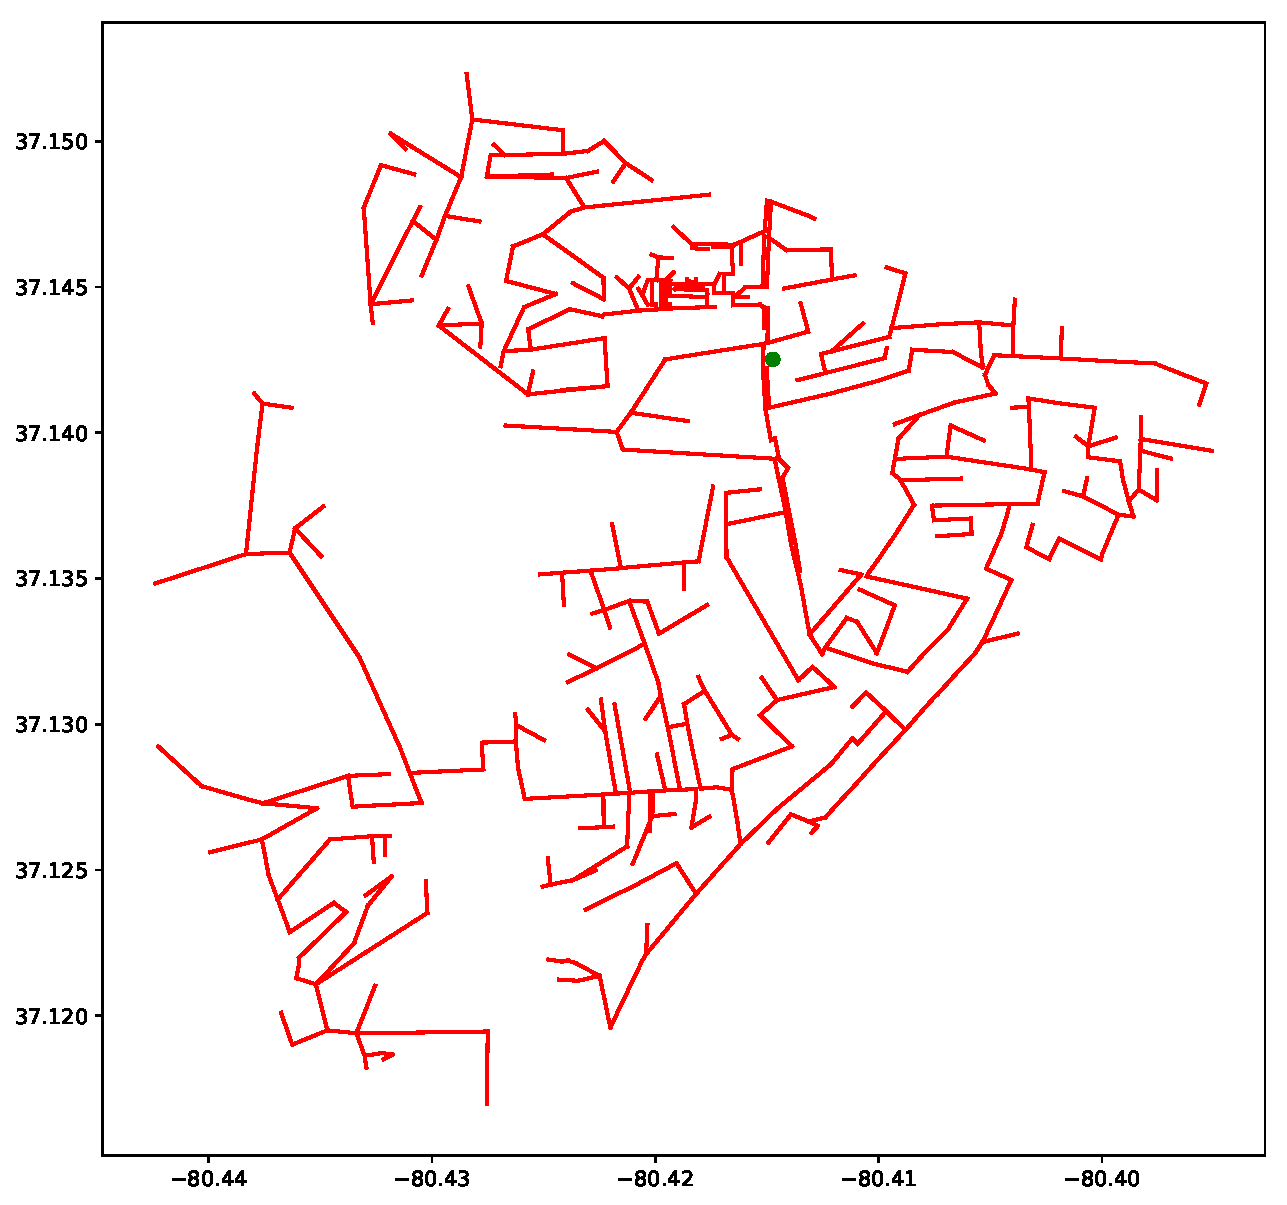
\includegraphics[scale=0.35]{figs/fig2b.pdf}
		\caption{Synthetic distribution network created using road network}
		\label{fig:2}
	\end{figure}
	
	It is seen from Fig.\ref{fig:2} that multiple sections of the road network do not have any home/activity locations mapped to them. Therefore, the distribution network need not follow the roadways in those sections. However, if the road nodes which are mapped to at least one home/activity location are only used to generate the radial distribution system as shown in Fig.\ref{fig:3}, it results in multiple isolated networks. There might be two primary reasons for such observation:
	\begin{enumerate}
		\item[(a)] The isolated set of distribution network (generated from the roadways) is actually supplied through the neighboring substation. However, the location of road nodes includes them in the Voronoi region of the selected substation. For example, in Fig.\ref{fig:3} the isolated set of edges at the bottom may be connected to the nodes present in the Voronoi region of another substation (different from ID $34816$). Therefore, differentiating nodes based on their location in the Voronoi region may not be an effective way to generate the synthetic distribution network.
		\item[(b)] Another possible reason for such isolated edges/nodes may be because the home/activity locations are mapped to road nodes and not the road edges. Many home/activity locations are located along the edges of road network, yet they are mapped to other road nodes (different from the nodes connected by the edges).
	\end{enumerate}
	
	\begin{figure}
		\centering
		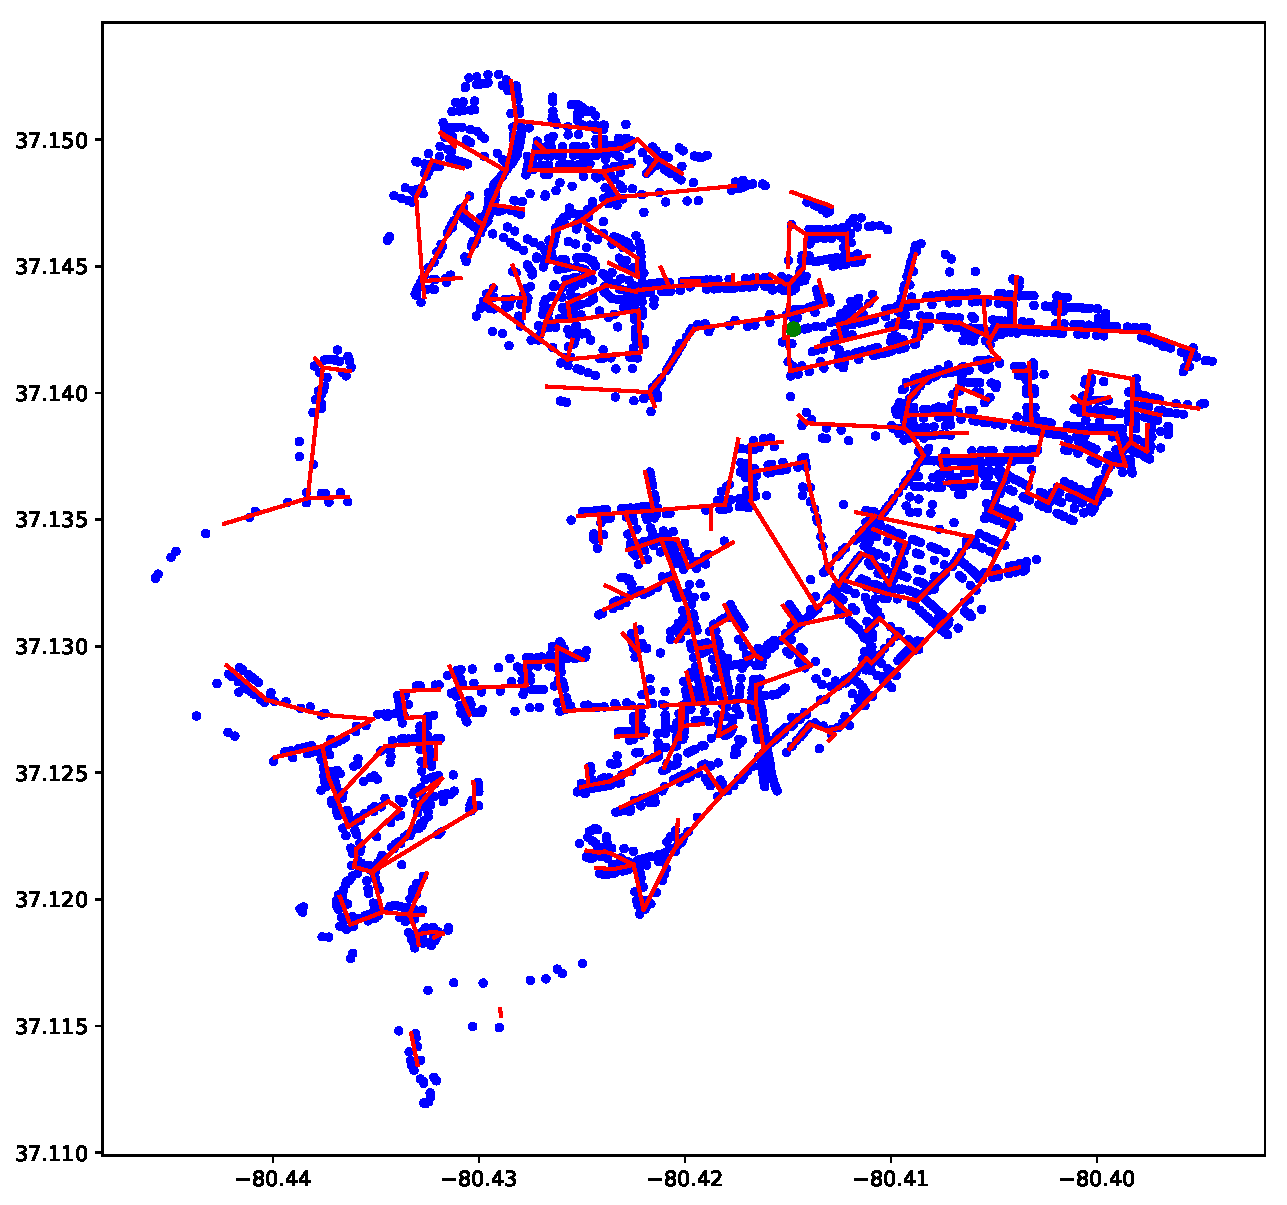
\includegraphics[scale=0.4]{figs/fig3.pdf}
		\caption{Synthetic distribution network created from road nodes mapped to home/activity locations}
		\label{fig:3}
	\end{figure} 
	
	\noindent
	\textbf{Algorithm.} Let $H$ denote the set of activity locations (e.g., homes, work locations). Let $R=(V_R,E_R)$ be a graph representation of the road network, where $V_R$ denotes its set of nodes (e.g., intersections, places where road structure changes), and where $E_R$ denotes its edges (also referred to as links.) Each link has associated an integer level from the set $\{1,2,3,4,5\}$ that describes the link type (e.g., a level-1 link could correspond to an Interstate road segment, while a level-5 link could correspond to a residential road.) Let $S$ denote the set of substations.
		
	The algorithm steps can be listed as follows:
	\begin{enumerate}
		\item From the set of links $E_R$, remove all links with level $\leq2$. These links are dropped since components of the distribution network (e.g., homes) are typically not located along these links.
		\item Construct a mapping $g:S\rightarrow V_R$ assigning to each substation $s\in S$ its closest (least \textit{great circle distance}) road node $g(s)\in V_R$. Let $N$ denote the set of all road nodes $g(s)$. $N=\{g(s),s\in S\}$. Thus, the set $N$ denotes the set of road network nodes which are closest to the substations.
		\item Calculate the network distance between points $(v,n)$ where $v\in V_R$ and $n\in N$ and construct a mapping $h:V_R\rightarrow N$ assigning to each node $v\in V_R$ its closest (least distance in the network) road node $h(v)\in N$. Therefore, it indirectly maps each point in the road network to the substations.
		\item Using depth first search (DFS) algorithm over over $V_R$,construct the connected components of the network $R$. Let $\mathcal{F}=\{T_1,T_2,\cdots\}$ denote the resulting forest of DFS trees.
		\item For each tree $T_i$, the DFS is performed by selecting the root node as $v\in N$ which is the nearest road node to the substation $s\in S$.
		\item Construct a mapping $f:H\rightarrow V_R$ assigning to each location $h \in H$ its closest node
		$f(h) \in V_R$. For each node $v \in V_R$, let $A(v)$ denote the set of locations mapped to $v$,
		and let $V\subset R = {v : A(v) \neq \phi}$ denote the subset of $V_R$ which have locations mapped to
		them (i.e., $f(H)$.). This creates a mapping between the road nodes and the activity nodes.
	\end{enumerate}
	
	\noindent
	\textbf{Results.} Using the above algorithm, the distribution network of Blacksburg, VA (zip code 24060) is generated as shown in Fig.\ref{fig:4}. The green circles denote the $9$ substations in Blacksburg. The red lines indicate the distribution network and the blue dots represent the activity locations. The yellow lines in Fig.\ref{fig:4} represent the map between the activity locations and the nearby road nodes.
	
	\begin{figure}
		\centering
		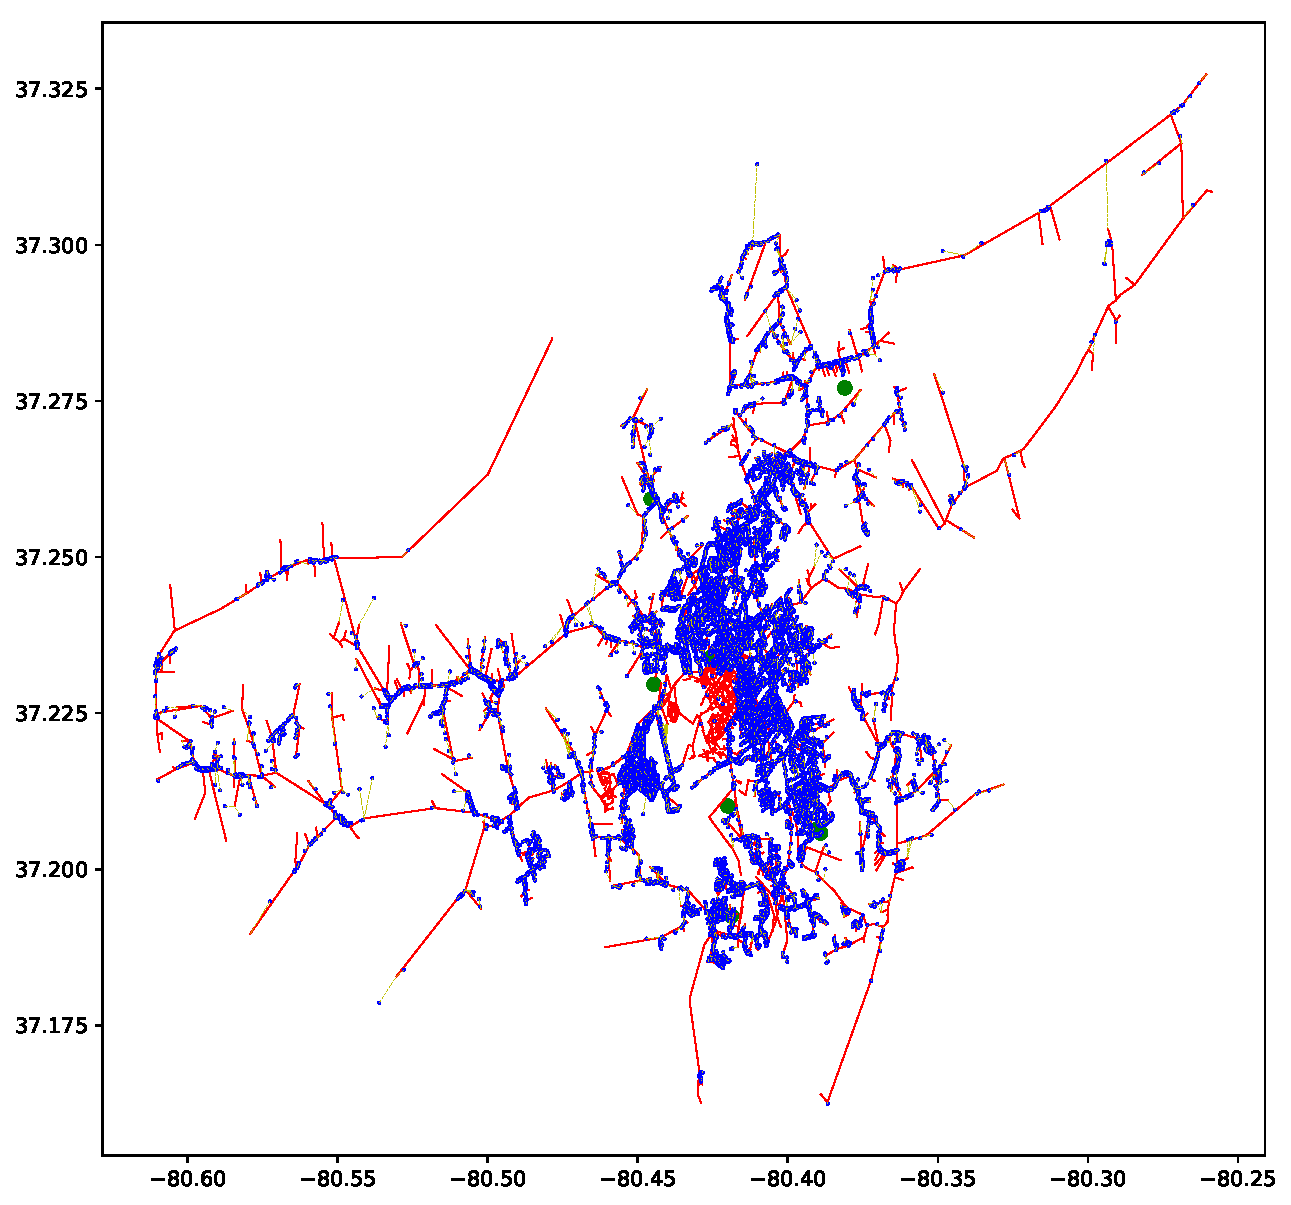
\includegraphics[scale=0.75]{figs/fig4.pdf}
		\caption{Synthetic distribution network of Blacksburg}
		\label{fig:4}
	\end{figure}
	
	\textbf{Comment 1:} The road network forms a single connected component if all the links are included in the graph. However, removing Level 1 and 2 links creates multiple components in the road network. Furthermore, some road networks in the area under consideration (Montgomery county) are extensions of road networks in the neighboring counties (e.g. Roanoke county). In such cases, the network distances of such road nodes from the substation nearby nodes are calculated as $\infty$ and the nodes are assigned to a random substation (in this case, it is substation with ID 34816).
	
	\textbf{Comment 2:} From Fig.\ref{fig:4} we also note there are multiple regions where the red predominates blue dots. This implies that there are no activity locations (blue) around such road nodes (red). An alternative needs to be formulated to avoid tracing road networks with no activity locations.
	
	\textbf{Comment3:} Fig.\ref{fig:5} represents the synthetic distribution network generated for the substation $34816$ (left) and for substation $28228$ (right). In either of the figures, we observe that some activity locations are located near to some edges; but mapped to nodes which are not close to those edges. To address this issue, the activity locations need to be mapped to the road links and not to the road nodes.
	\begin{figure}
		\centering
		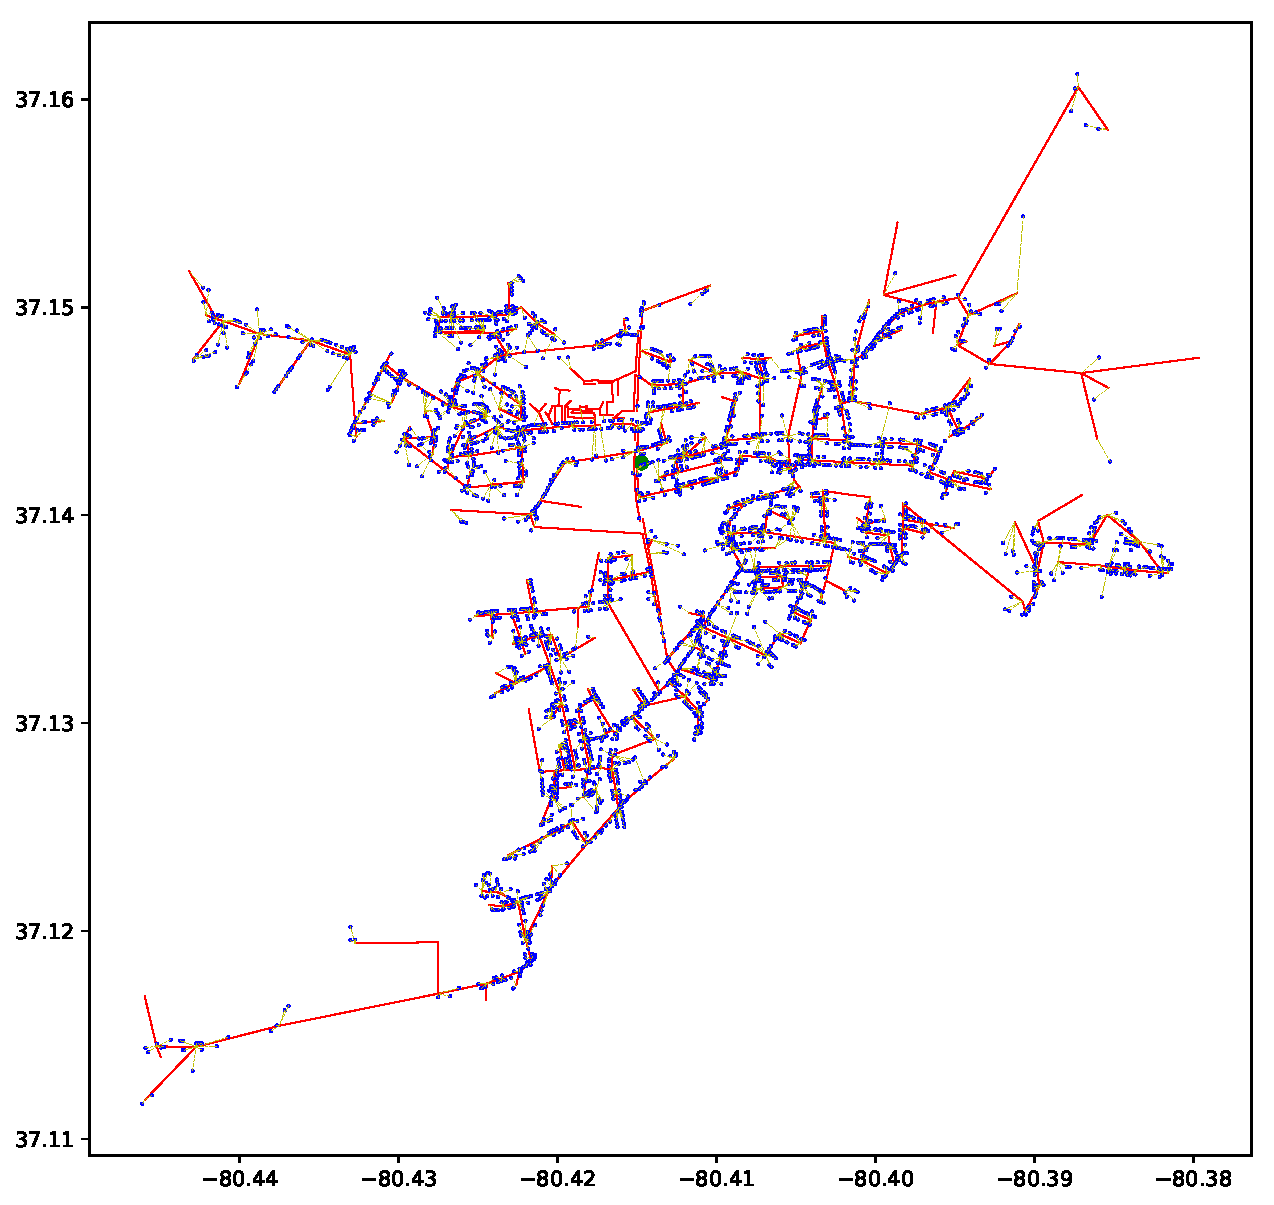
\includegraphics[scale=0.35]{figs/fig5a.pdf}
		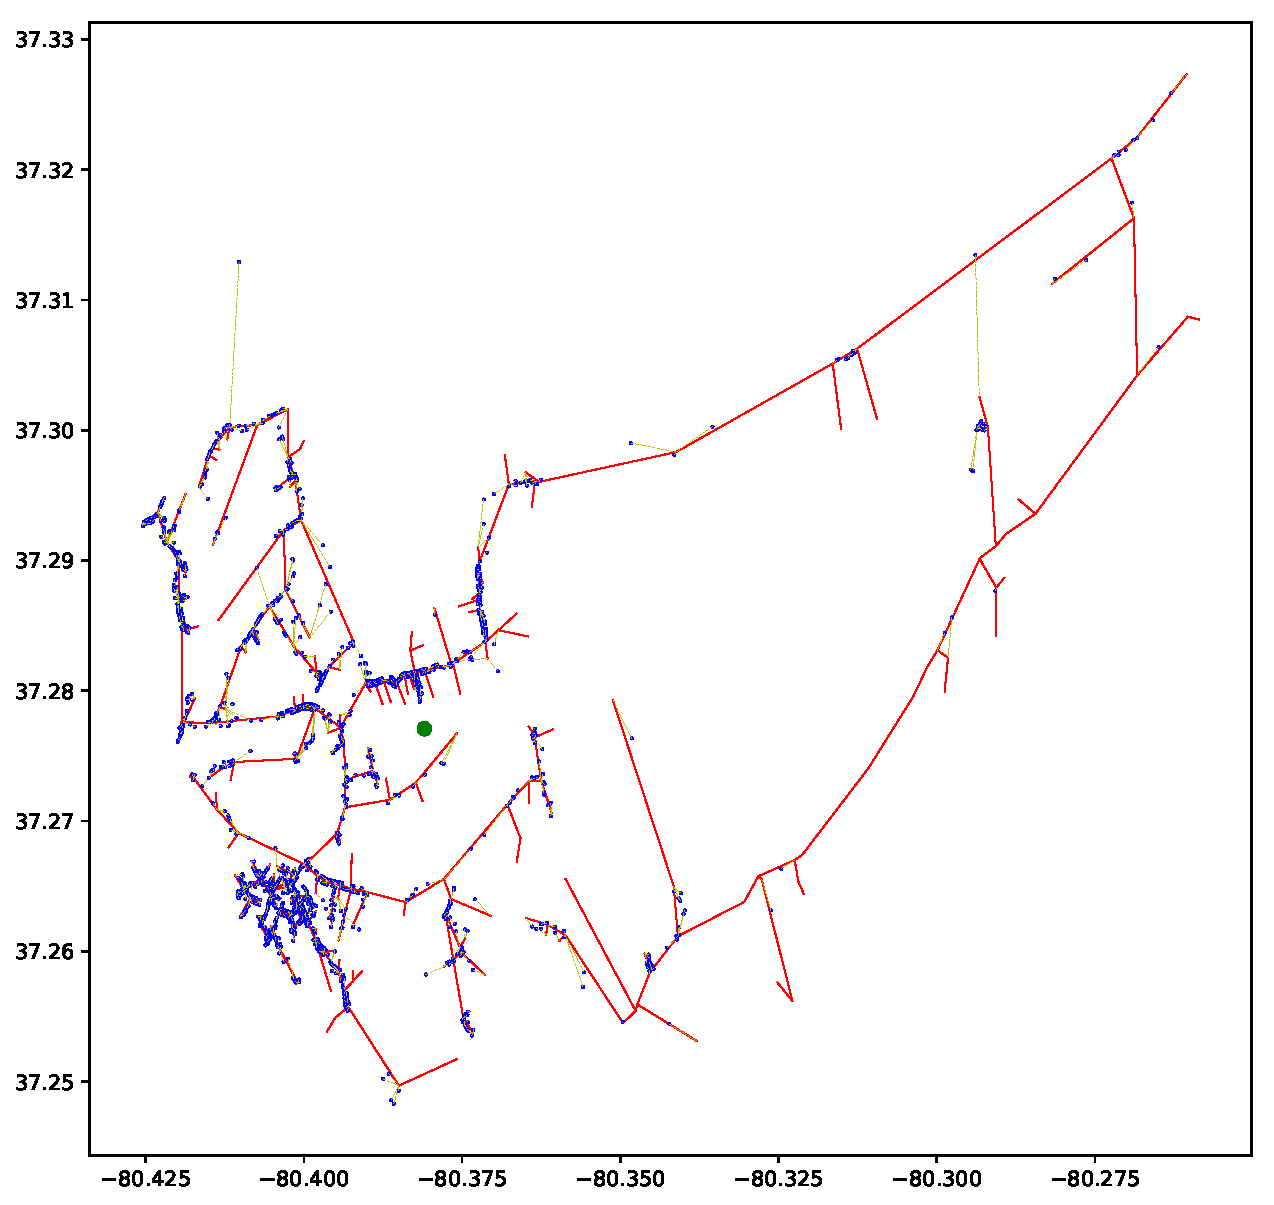
\includegraphics[scale=0.35]{figs/fig5b.pdf}
		\caption{Synthetic distribution network of two substations (left: 34816, right: 28228)}
		\label{fig:5}
	\end{figure}
\end{document}